
\vspace{0.75cm}

The includes needed
\begin{itemize}
    \item stdio.h : to printf and get user input
    \item stdlib.h : to use exit to terminate whole 
programe and to terminate child process
    \item unistd.h :to use fork and pipe primitive
    \item ctype.h : to use toupper function
    \item sys/wait.h : to use wait primitive (parent wait for child to terminate)
\end{itemize}
\newpage
\lstinputlisting[style=cstyle,basicstyle=\footnotesize\ttfamily]{Questions/EX1/ex1Overview.c}

child\_1 void function :
\lstinputlisting[style=cstyle,firstline=10,lastline=33,basicstyle=\footnotesize\ttfamily]{Questions/EX1/ex1.c}

\vspace{0.5cm}

child\_2 void function :
\lstinputlisting[style=cstyle,firstline=36,lastline=50,basicstyle=\footnotesize\ttfamily]{Questions/EX1/ex1.c}



\begin{center}
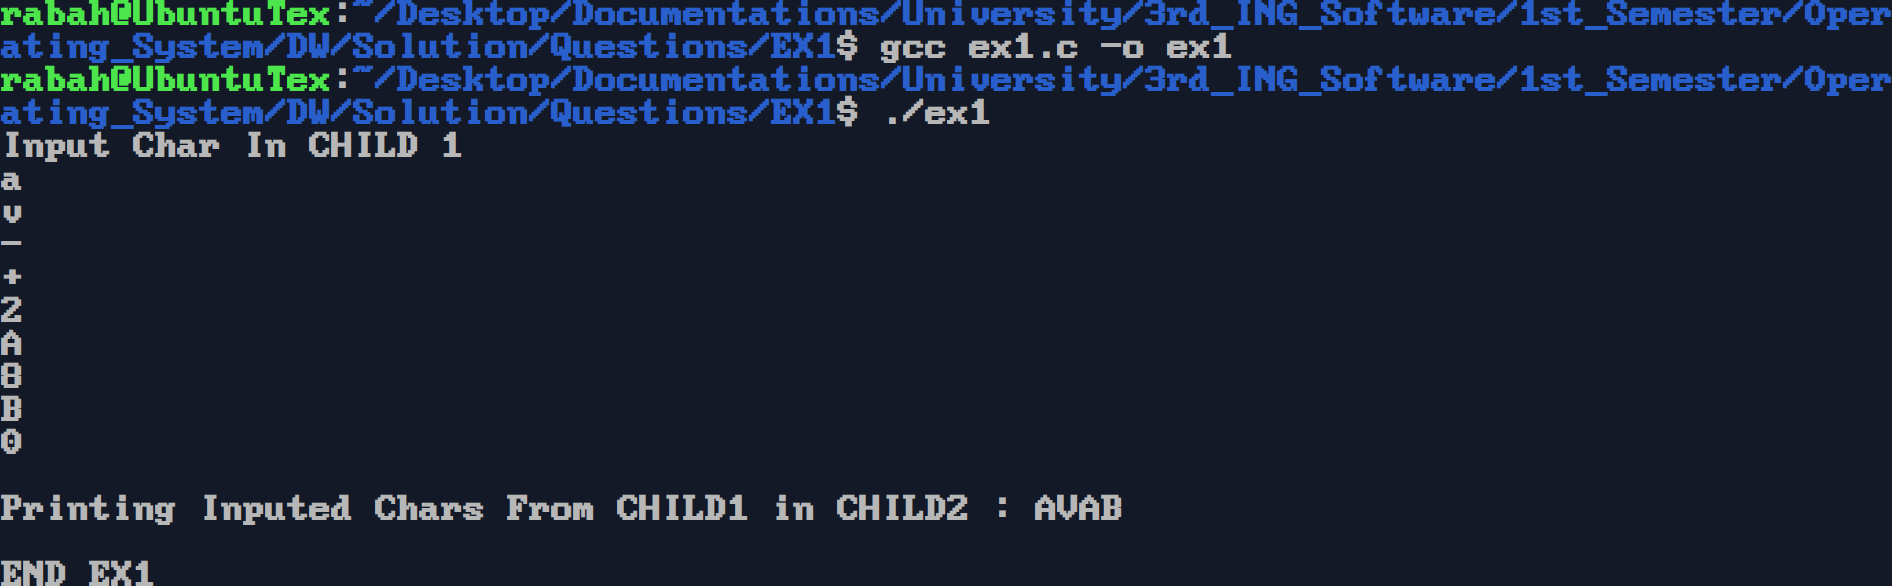
\includegraphics[width=\textwidth]{Questions/EX1/output.png}
\end{center}

